%!TeX encoding = UTF-8
%!TeX program = xelatex
\documentclass[
  notheorems,
  aspectratio=54,
]{beamer}

%% preamble
\title{Mathematical modelling of infectious diseases}
% \subtitle{The subtitle}
\author{Jingsheng Gao}
\institute{Anqing Normal University}

\useoutertheme{shadow}
\setbeamertemplate{headline}{}
\mode<presentation>{
  \usetheme{Warsaw}
  \usecolortheme{seagull}
}

\setbeamertemplate{footline}
{
  \leavevmode%
  \hbox{%
  \begin{beamercolorbox}[wd=.45\paperwidth,ht=2.25ex,dp=1ex,center]{title in head/foot}%
    \usebeamerfont{title in head/foot}\inserttitle
  \end{beamercolorbox}%
  \begin{beamercolorbox}[wd=.45\paperwidth,ht=2.25ex,dp=1ex,center]{author in head/foot}%
      \usebeamerfont{author in head/foot}\insertauthor\ - \insertinstitute
  \end{beamercolorbox}%
  \begin{beamercolorbox}[wd=.1\paperwidth,ht=2.25ex,dp=1ex,right]{date in head/foot}%
    \insertframenumber{} / \inserttotalframenumber\hspace*{2ex} 
  \end{beamercolorbox}}%
  \vskip0pt%
}


\setbeamertemplate{navigation symbols}{}

\usepackage[
    backend=biber,
    autocite=superscript,
    sorting=none
]{biblatex}
\AtBeginBibliography{\small}
\addbibresource{refs.bib}

\usepackage{caption}
\captionsetup[figure]{font=scriptsize}

\usepackage{latexsym}
\usepackage{amsmath,amssymb}
\usepackage{mathtools}
\usepackage{color,xcolor}
\usepackage{graphicx}
\usepackage{algorithm}
\usepackage{amsthm}
\usepackage{lmodern}
\usepackage[UTF8]{ctex}
\usepackage{xeCJK}
\usepackage{animate} % insert gif

\usepackage{lipsum}
\usepackage{ulem}

\usepackage{listings} % display code on slides; don't forget [fragile] option after \begin{frame}

% ----------------------------------------------
% tikx
\usepackage{framed}
\usepackage{tikz}
\usepackage{pgf}
\usetikzlibrary{calc,trees,positioning,arrows,chains,shapes.geometric,%
    decorations.pathreplacing,decorations.pathmorphing,shapes,%
    matrix,shapes.symbols}



% ----------------------------------------------

% ---------------------------------------------------------------------
% Jet Black Theme
% \setbeamercolor{normal text}{fg=white,bg=black!90}
% \setbeamercolor{structure}{fg=white}
%
% \setbeamercolor{alerted text}{fg=red!85!black}
%
% \setbeamercolor{item projected}{use=item,fg=black,bg=item.fg!35}
%
% \setbeamercolor*{palette primary}{use=structure,fg=structure.fg}
% \setbeamercolor*{palette secondary}{use=structure,fg=structure.fg!95!black}
% \setbeamercolor*{palette tertiary}{use=structure,fg=structure.fg!90!black}
% \setbeamercolor*{palette quaternary}{use=structure,fg=structure.fg!95!black,bg=black!80}
%
% \setbeamercolor*{framesubtitle}{fg=white}
%
% \setbeamercolor*{block title}{parent=structure,bg=black!70!gray}
% \setbeamercolor*{block body}{fg=black,bg=black!10}
% \setbeamercolor*{block title alerted}{parent=alerted text,bg=black!15}
% \setbeamercolor*{block title example}{parent=example text,bg=black!15}
% ---------------------------------------------------------------------


% \newcommand{\reditem}[1]{\setbeamercolor{item}{fg=red}\item #1}

% \newcommand*{\Scale}[2][4]{\scalebox{#1}{\ensuremath{#2}}}

% -------------------------------------------------------------

% -------------------------------------------------------------

\begin{document}

% title frame
\begin{frame}
    \titlepage
\end{frame}

\begin{frame}{Introduction}
 \begin{itemize}
    \item Mathematical models can project how infectious diseases progress to show the likely outcome of an epidemic (including in plants) and help inform public health and plant health interventions. 数学模型可以预测传染病的进展情况,以显示流行病(包括植物中)的可能结果,并帮助为公共卫生和植物健康干预措施提供信息。
    \item Models use basic assumptions or collected statistics along with mathematics to find parameters for various infectious diseases and use those parameters to calculate the effects of different interventions, like mass vaccination programs. 模型使用基本假设或收集的统计数据以及数学来查找各种传染病的参数,并使用这些参数来计算不同干预措施(例如大规模疫苗接种计划)的效果。
  \end{itemize}
\end{frame}

\begin{frame}{History}
  \begin{figure}
    \centering
  \end{figure}
  \begin{itemize}
    \item The modelling of infectious diseases is a tool that has been used to study the mechanisms by which diseases spread, to predict the future course of an outbreak and to evaluate strategies to control an epidemic. 传染病建模是一种用于研究疾病传播机制、预测未来爆发过程以及评估控制流行病策略的工具。
    \item The first scientist who systematically tried to quantify causes of death was John Graunt in his book Natural and Political Observations made upon the Bills of Mortality, in 1662. 第一位系统地尝试量化死亡原因的科学家是约翰·格朗特 (John Graunt),他于 1662 年在其著作《自然和政治观察》中对死亡率进行了观察。
    \item The earliest account of mathematical modelling of spread of disease was carried out in 1760 by Daniel Bernoulli. 丹尼尔·伯努利 (Daniel Bernoulli) 于 1760 年对疾病传播的数学模型进行了最早的描述。
  \end{itemize}
\end{frame}

\begin{frame}{History}
  \begin{figure}
    \centering
  \end{figure}
  \begin{itemize}
    \item In the early 20th century, William Hamer and Ronald Ross applied the law of mass action to explain epidemic behaviour. 20世纪初,威廉·哈默和罗纳德·罗斯应用群体行动定律来解释流行病行为。
    \item The 1920s saw the emergence of compartmental models. The Kermack–McKendrick epidemic model (1927) and the Reed–Frost epidemic model (1928) both describe the relationship between susceptible, infected and immune individuals in a population. 20 年代出现了隔间模型。 Kermack-McKendrick 流行病模型 (1927) 和 Reed-Frost 流行病模型 (1928) 都描述了人群中易感者、感染者和免疫个体之间的关系。
  \end{itemize}
\end{frame}

\begin{frame}{History}
  \begin{figure}
    \centering
  \end{figure}
  \begin{itemize}
    \item Recently, agent-based models (ABMs) have been used in exchange for simpler compartmental models. For example, epidemiological ABMs have been used to inform public health (nonpharmaceutical) interventions against the spread of SARS-CoV-2. 最近,基于代理的模型(ABM)已被用来代替更简单的分区模型。 例如,流行病学 ABM 已被用来为针对 SARS-CoV-2 传播的公共卫生(非药物)干预措施提供信息。
  \end{itemize}
\end{frame}

\begin{frame}{Assumptions}
  \begin{itemize}
    \item Models are only as good as the assumptions on which they are based. If a model makes predictions that are out of line with observed results and the mathematics is correct, the initial assumptions must change to make the model useful. 模型的好坏取决于它们所基于的假设。如果模型做出的预测与观察到的结果不一致并且数学是正确的,则必须更改初始假设以使模型有用
  \end{itemize}
\end{frame}

\begin{frame}{Assumptions}
  \begin{itemize}
    \item Rectangular and stationary age distribution, i.e., everybody in the population lives to age L and then dies, and for each age (up to L) there is the same number of people in the population. 矩形且固定的年龄分布,即人口中的每个人都活到 L 岁然后死亡,并且对于每个年龄(直到 L)人口中的人数相同。
  \begin{figure}
    \centering
    \textbf{Examples}\par\medskip
    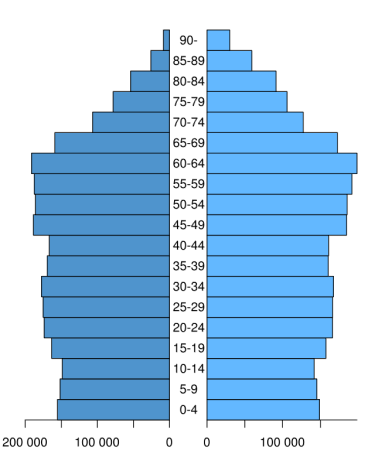
\includegraphics[width=0.4\textwidth]{age_distribution.png}
  \end{figure}
  \end{itemize}
\end{frame}

\begin{frame}{Assumptions}
  \begin{itemize}
    \item Homogeneous mixing of the population, i.e., individuals of the population under scrutiny assort and make contact at random and do not mix mostly in a smaller subgroup. This assumption is rarely justified because social structure is widespread. 群体的同质混合,即,受审查的群体中的个体随机分类和接触,并且不会在较小的子群体中大部分混合。这种假设很少成立,因为社会结构很普遍。
  \end{itemize}
\end{frame}

\begin{frame}{Types of epidemic models - Stochastic}
  \begin{itemize}
    \item "Stochastic" means being or having a random variable. A stochastic model is a tool for estimating probability distributions of potential outcomes by allowing for random variation in one or more inputs over time. Stochastic models depend on the chance variations in risk of exposure, disease and other illness dynamics. Statistical agent-level disease dissemination in small or large populations can be determined by stochastic methods. “随机”是指存在或具有随机变量。随机模型是一种通过允许一个或多个输入随时间的随机变化来估计潜在结果的概率分布的工具。随机模型取决于暴露风险、疾病和其他疾病动态的机会变化。可以通过随机方法确定小群体或大群体中统计代理水平的疾病传播。
  \end{itemize}
\end{frame}

\begin{frame}{Types of epidemic models - Deterministic}
  \begin{itemize}
    \item When dealing with large populations, as in the case of tuberculosis, deterministic or compartmental mathematical models are often used. In a deterministic model, individuals in the population are assigned to different subgroups or compartments, each representing a specific stage of the epidemic. 在处理大量人群时,例如结核病,通常使用确定性或区室数学模型。在确定性模型中,群体中的个体被分配到不同的亚组或区室,每个亚组或区室代表流行病的特定阶段。
  \end{itemize}
\end{frame}

\begin{frame}{Types of epidemic models - Deterministic}
  \begin{itemize}
    \item The transition rates from one class to another are mathematically expressed as derivatives, hence the model is formulated using differential equations. While building such models, it must be assumed that the population size in a compartment is differentiable with respect to time and that the epidemic process is deterministic. In other words, the changes in population of a compartment can be calculated using only the history that was used to develop the model. 从一类到另一类的转换率在数学上表示为导数,因此该模型是使用微分方程制定的。在构建此类模型时,必须假设隔间中的人口规模相对于时间是可微的,并且流行病过程是确定性的。换句话说,可以仅使用用于开发模型的历史来计算隔间的人口变化。
  \end{itemize}
\end{frame}

\begin{frame}{Reproduction number}
  \begin{itemize}
    \item The basic reproduction number (denoted by R0) is a measure of how transferable a disease is. It is the average number of people that a single infectious person will infect over the course of their infection. 基本传染数(用 R0 表示)是衡量疾病传染性的指标。这是单个感染者在感染过程中平均感染的人数。
    \item This quantity determines whether the infection will increase sub-exponentially, die out, or remain constant: if R0 > 1, then each person on average infects more than one other person so the disease will spread; if R0 < 1, then each person infects fewer than one person on average so the disease will die out; and if R0 = 1, then each person will infect on average exactly one other person, so the disease will become endemic: it will move throughout the population but not increase or decrease.
  \end{itemize}
\end{frame}

\begin{frame}{Reproduction number - Endemic steady state}
  \begin{itemize}
    \item An infectious disease is said to be endemic when it can be sustained in a population without the need for external inputs. This means that, on average, each infected person is infecting exactly one other person (any more and the number of people infected will grow sub-exponentially and there will be an epidemic, any less and the disease will die out). In mathematical terms, that is: 
      $${\displaystyle \ R_{0}S\ =1}.$$
    The basic reproduction number (R0) of the disease, assuming everyone is susceptible, multiplied by the proportion of the population that is actually susceptible (S) must be one (since those who are not susceptible do not feature in our calculations as they cannot contract the disease).
  \end{itemize}
\end{frame}

\begin{frame}{Reproduction number - Endemic steady state}
  Assume the rectangular stationary age distribution and let also the ages of infection have the same distribution for each birth year. Let the average age of infection be A, for instance when individuals younger than A are susceptible and those older than A are immune (or infectious). Then it can be shown by an easy argument that the proportion of the population that is susceptible is given by:
${\displaystyle S={\frac {A}{L}}.}$
We reiterate that L is the age at which in this model every individual is assumed to die. But the mathematical definition of the endemic steady state can be rearranged to give:
${\displaystyle S={\frac {1}{R_{0}}}.}$
Therefore, due to the transitive property:
${\displaystyle {\frac {1}{R_{0}}}={\frac {A}{L}}\Rightarrow R_{0}={\frac {L}{A}}.}$
This provides a simple way to estimate the parameter R0 using easily available data.

For a population with an exponential age distribution,
${\displaystyle R_{0}=1+{\frac {L}{A}}.}$
This allows for the basic reproduction number of a disease given A and L in either type of population distribution.
\end{frame}


\begin{frame}{Sub-exponential growth}
  \begin{itemize}
    \item A common explanation for the growth of epidemics holds that 1 person infects 2, those 2 infect 4 and so on and so on with the number of infected doubling every generation. 对于流行病蔓延的一个常见解释是,1 人感染 2 人,2 人感染 4 人,以此类推,感染人数每一代都会翻倍。
    \item  Thus this model of an epidemic leads to a curve that grows exponentially until it crashes to zero as all the population have been infected. i.e. no herd immunity and no peak and gradual decline as seen in reality. 因此,这种流行病模型导致曲线呈指数增长,直到所有人口都被感染时曲线崩溃至零。即没有群体免疫,也没有现实中看到的峰值和逐渐下降。
  \end{itemize}
\end{frame}

\begin{frame}{Sub-exponential growth - Epidemic Models on Networks}
  \begin{itemize}
    \item Epidemics can be modeled as diseases spreading over networks of contact between people. Such a network can be represented mathematically with a graph and is called the contact network. 流行病可以被建模为通过人与人之间的接触网络传播的疾病。这样的网络可以用图形在数学上表示,称为接触网络。
    \item Every node in a contact network is a representation of an individual and each link (edge) between a pair of nodes represents the contact between them. 接触网络中的每个节点都代表一个个体,一对节点之间的每个链接(边)代表它们之间的接触。
  \end{itemize}
\end{frame}

\begin{frame}{Sub-exponential growth - Epidemic Models on Networks}
  \begin{itemize}
    \item Links in the contact networks may be used to transmit the disease between the individuals and each disease has its own dynamics on top of its contact network. 接触网络中的链接可用于在个体之间传播疾病,并且每种疾病在其接触网络之上都有其自己的动态。
    \item The combination of disease dynamics under the influence of interventions, if any, on a contact network may be modeled with another network, known as a transmission network. 接触网络上的干预措施(如果有的话)影响下的疾病动态组合可以用另一个网络(称为传播网络)进行建模。
    \item  In a transmission network, all the links are responsible for transmitting the disease. 在传播网络中,所有环节都负责传播疾病。
  \end{itemize}
\end{frame}

\begin{frame}{Sub-exponential growth - Epidemic Models on Networks}
  \begin{itemize}
    \item If such a network is a locally tree-like network, meaning that any local neighborhood in such a network takes the form of a tree, then the basic reproduction can be written in terms of the average excess degree of the transmission network such that: 如果这样的网络是局部树状网络,意味着这样的网络中的任何局部邻域都采用树的形式,那么基本再现可以用传输网络的平均过剩度来写,这样:
      $$ {\displaystyle R_{0}={\frac {\langle k^{2}\rangle }{\langle k\rangle }}-1}, $$
    where 
${\displaystyle {\langle k\rangle }}$ is the mean-degree (average degree) of the network and 
${\displaystyle {\langle k^{2}\rangle }}$ is the second moment of the transmission network degree distribution.
It is, however, not always straightforward to find the transmission network out of the contact network and the disease dynamics.
  \end{itemize}
\end{frame}

\begin{frame}{Sub-exponential growth}
  \begin{center}
  Video
  \end{center}
\end{frame}

\begin{frame}{Sub-exponential growth - Epidemic Models on Networks}
  \begin{itemize}
    \item For example, if a contact network can be approximated with an Erdős–Rényi graph with a Poissonian degree distribution, and the disease spreading parameters are as defined in the example above, such that
${\displaystyle \beta }$ is the transmission rate per person and the disease has a mean infectious period of
${\displaystyle {\dfrac {1}{\gamma }}}$, then the basic reproduction number is
${\displaystyle R_{0}={\dfrac {\beta }{\gamma }}{\langle k\rangle }}$ since
${\displaystyle {\langle k^{2}\rangle }-{\langle k\rangle }^{2}={\langle k\rangle }}$ for a Poisson distribution.
  \end{itemize}
\end{frame}

\begin{frame}{Compartmental models in epidemiology}
  \begin{itemize}
    \item Compartmental models are formulated as Markov chains. A classic compartmental model in epidemiology is the SIR model, which may be used as a simple model for modelling epidemics. Multiple other types of compartmental models are also employed. 房室模型被表述为马尔可夫链。流行病学中的经典区室模型是 SIR 模型,它可以用作流行病建模的简单模型。还采用了多种其他类型的隔室模型。
    \item There are many modifications of the SIR model, including those that include births and deaths, where upon recovery there is no immunity (SIS model), where immunity lasts only for a short period of time (SIRS), where there is a latent period of the disease where the person is not infectious (SEIS and SEIR), and where infants can be born with immunity (MSIR).
  \end{itemize}
\end{frame}

\begin{frame}{Compartmental models in epidemiology - The SIR model}
    In 1927, W. O. Kermack and A. G. McKendrick created a model in which they considered a fixed population with only three compartments: susceptible, 
${\displaystyle S(t)}$; infected, 
${\displaystyle I(t)}$; and recovered, 
${\displaystyle R(t)}$. The compartments used for this model consist of three classes:
  \begin{itemize}
    \item ${\displaystyle S(t)}$ is used to represent the individuals not yet infected with the disease at time t, or those susceptible to the disease of the population.
    \item ${\displaystyle I(t)}$ denotes the individuals of the population who have been infected with the disease and are capable of spreading the disease to those in the susceptible category.
    \item ${\displaystyle R(t)}$ is the compartment used for the individuals of the population who have been infected and then removed from the disease, either due to immunization or due to death. Those in this category are not able to be infected again or to transmit the infection to others.
  \end{itemize}
\end{frame}

\begin{frame}{Compartmental models in epidemiology - The SIR model}
  \begin{center}
  Video
  \end{center}
\end{frame}

\begin{frame}{The SIR model - Transition rates}
  \begin{itemize}
    \item Between S and I, the transition rate is assumed to be 
${\displaystyle d(S/N)/dt=-\beta SI/N^{2}}$, where 
${\displaystyle N}$ is the total population, 
${\displaystyle \beta }$ is the average number of contacts per person per time, multiplied by the probability of disease transmission in a contact between a susceptible and an infectious subject, and 
${\displaystyle SI/N^{2}}$ is the fraction of those contacts between an infectious and susceptible individual which result in the susceptible person becoming infected.

  \item Between I and R, the transition rate is assumed to be proportional to the number of infectious individuals which is 
${\displaystyle \gamma I}$. If an individual is infectious for an average time period 
${\displaystyle D}$, then 
${\displaystyle \gamma =1/D}$.
This is also equivalent to the assumption that the length of time spent by an individual in the infectious state is a random variable with an exponential distribution.
  \end{itemize}
\end{frame}


\begin{frame}{The SIR model without birth and death}
  The dynamics of an epidemic, for example, the flu, are often much faster than the dynamics of birth and death, therefore, birth and death are often omitted in simple compartmental models. The SIR system without so-called vital dynamics (birth and death, sometimes called demography) described above can be expressed by the following system of ordinary differential equations:
  $${\displaystyle \left\{{\begin{aligned}&{\frac {dS}{dt}}=-{\frac {\beta IS}{N}},\\[6pt]&{\frac {dI}{dt}}={\frac {\beta IS}{N}}-\gamma I,\\[6pt]&{\frac {dR}{dt}}=\gamma I,\end{aligned}}\right.}$$
    where 
${\displaystyle S}$ is the stock of susceptible population, 
${\displaystyle I}$ is the stock of infected, 
${\displaystyle R}$ is the stock of removed population (either by death or recovery), and
${\displaystyle N}$ is the sum of these three.
\end{frame}

\begin{frame}{Mathematics of mass vaccination}
  If the proportion of the population that is immune exceeds the herd immunity level for the disease, then the disease can no longer persist in the population and its transmission dies out. Thus, a disease can be eliminated from a population if enough individuals are immune due to either vaccination or recovery from prior exposure to disease. For example, smallpox eradication, with the last wild case in 1977, and certification of the eradication of indigenous transmission of 2 of the 3 types of wild poliovirus (type 2 in 2015, after the last reported case in 1999, and type 3 in 2019, after the last reported case in 2012). 如果免疫的人口比例超过了对该疾病的群体免疫水平,那么该疾病就无法再在人群中持续存在,其传播就会消失。 因此,如果有足够多的个体因疫苗接种或从先前接触疾病中恢复而获得免疫力,则可以从人群中消除疾病。例如,消灭天花,最后一个野生病例发生在 1977 年,并认证消灭了 3 种野生脊髓灰质炎病毒中的 2 种本土传播(2 型于 2015 年,在 1999 年报告了最后一个病例之后,3 型于 2019 年) ,继 2012 年最后一次报告病例之后)。
\end{frame}

\begin{frame}{Mathematics of mass vaccination}
  The herd immunity level will be denoted q. Recall that, for a stable state:
$${\displaystyle R_{0}\cdot S=1.}$$
In turn,
$${\displaystyle R_{0}={\frac {N}{S}}={\frac {\mu N\operatorname {E} (T_{L})}{\mu N\operatorname {E} [\min(T_{L},T_{S})]}}={\frac {\operatorname {E} (T_{L})}{\operatorname {E} [\min(T_{L},T_{S})]}},}$$
which is approximately:
$${\displaystyle {\frac {\operatorname {\operatorname {E} } (T_{L})}{\operatorname {\operatorname {E} } (T_{S})}}=1+{\frac {\lambda }{\mu }}={\frac {\beta N}{v}}.}$$
\end{frame}

\begin{frame}{Mathematics of mass vaccination}
S will be (1 − q), since q is the proportion of the population that is immune and q + S must equal one (since in this simplified model, everyone is either susceptible or immune). Then:
$${\displaystyle {\begin{aligned}&R_{0}\cdot (1-q)=1,\\[6pt]&1-q={\frac {1}{R_{0}}},\\[6pt]&q=1-{\frac {1}{R_{0}}}.\end{aligned}}}$$
  Remember that this is the threshold level. Die out of transmission will only occur if the proportion of immune individuals exceeds this level due to a mass vaccination programme.
\end{frame}

\begin{frame}{Mathematics of mass vaccination}
  We have just calculated the critical immunization threshold (denoted qc). It is the minimum proportion of the population that must be immunized at birth (or close to birth) in order for the infection to die out in the population.
$${\displaystyle q_{c}=1-{\frac {1}{R_{0}}}.}$$
Because the fraction of the final size of the population p that is never infected can be defined as:
$${\displaystyle \lim _{t\to \infty }S(t)=e^{-\int _{0}^{\infty }\lambda (t)\,dt}=1-p.}$$
Hence,
$${\displaystyle p=1-e^{-\int _{0}^{\infty }\beta I(t)\,dt}=1-e^{-R_{0}p}.}$$
Solving for 
${\displaystyle R_{0}}$, we obtain:
$${\displaystyle R_{0}={\frac {-\ln(1-p)}{p}}.}$$
\end{frame}

\begin{frame}{When mass vaccination cannot exceed the herd immunity}
  If the vaccine used is insufficiently effective or the required coverage cannot be reached, the program may fail to exceed qc. Such a program will protect vaccinated individuals from disease, but may change the dynamics of transmission.[citation needed]

Suppose that a proportion of the population q (where q < qc) is immunised at birth against an infection with R0 > 1. The vaccination programme changes R0 to Rq where
$${\displaystyle R_{q}=R_{0}(1-q)}$$
This change occurs simply because there are now fewer susceptibles in the population who can be infected. Rq is simply R0 minus those that would normally be infected but that cannot be now since they are immune.
\end{frame}

\begin{frame}{When mass vaccination cannot exceed the herd immunity}
  As a consequence of this lower basic reproduction number, the average age of infection A will also change to some new value Aq in those who have been left unvaccinated.

Recall the relation that linked R0, A and L. Assuming that life expectancy has not changed, now:
$${\displaystyle R_{q}={\frac {L}{A_{q}}},}$$
$${\displaystyle A_{q}={\frac {L}{R_{q}}}={\frac {L}{R_{0}(1-q)}}.}$$
But R0 = L/A so:
$${\displaystyle A_{q}={\frac {L}{(L/A)(1-q)}}={\frac {AL}{L(1-q)}}={\frac {A}{1-q}}.}$$
\end{frame}

\begin{frame}{When mass vaccination cannot exceed the herd immunity}
Thus, the vaccination program may raise the average age of infection, and unvaccinated individuals will experience a reduced force of infection due to the presence of the vaccinated group. For a disease that leads to greater clinical severity in older populations, the unvaccinated proportion of the population may experience the disease relatively later in life than would occur in the absence of vaccine. 因此,疫苗接种计划可能会提高平均感染年龄,而未接种疫苗的个体将因接种疫苗群体的存在而降低感染力。对于在老年人群中导致更严重的临床严重性的疾病,未接种疫苗的人口比例可能比没有疫苗的情况下相对较晚地罹患该疾病。
\end{frame}

\begin{frame}{When mass vaccination exceeds the herd immunity}
  If a vaccination program causes the proportion of immune individuals in a population to exceed the critical threshold for a significant length of time, transmission of the infectious disease in that population will stop. If elimination occurs everywhere at the same time, then this can lead to eradication. 如果疫苗接种计划导致人群中免疫个体的比例在相当长的时间内超过临界阈值,那么该人群中传染病的传播就会停止。如果消除同时在各处发生,那么这可能会导致根除。
\end{frame}

\begin{frame}{When mass vaccination exceeds the herd immunity}
  \begin{itemize}
    \item Elimination - 
      Interruption of endemic transmission of an infectious disease, which occurs if each infected individual infects less than one other, is achieved by maintaining vaccination coverage to keep the proportion of immune individuals above the critical immunization threshold. 通过维持疫苗接种覆盖率,使免疫个体的比例保持在临界免疫阈值以上,可以阻断传染病的地方性传播(如果每个受感染者的感染人数少于其他人)。
    \item Eradication - 
      Elimination everywhere at the same time such that the infectious agent dies out (for example, smallpox and rinderpest). 同时消除各处,使传染源消失(例如天花和牛瘟)。
  \end{itemize}
\end{frame}

\nocite{*}
\begin{frame}{References}
    \printbibliography
\end{frame}

\begin{frame}{}
  \centering \Huge
  \emph{Thanks for listening!}
\end{frame}

\end{document}



